\documentclass[
a4paper,
10pt,
twoside,
prd,
aps,
nofootinbib,
superscriptaddress,
floatfix,
preprintnumbers,
]{article}


\usepackage{preamble}
\usepackage{titleinfo}

\geometry{ % Set document margins
	top     = 2cm,
	bottom  = 2cm,
	left    = 1cm,
	right   = 1cm
}

\newcommand{\mcols}{1} % Choose number of columns (>= 1)


\bibSetup{refs.bib} % Give references file 
% ===== Format headers & footers =====

\pagestyle{fancy}
\fancyhf{}
\fancyhead[LE,RO]{B. Henke}
\fancyhead[LO]{\headertitle\hspace{0.5cm}\textit{PHY803}}
\fancyhead[RE]{\textit{PHY803}\hspace{0.5cm}\headertitle}
\fancyfoot[RE,LO]{\thepage}

\begin{document}
% \tableofcontents
\titleinf
\maketitle \startmcols

\section{}
\subsection{}
\begin{figure}[H]
	\centering
	\begin{subfigure}[a]{\linewidth}
		\centering
		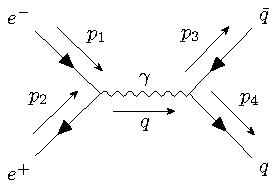
\includegraphics[width=0.3375\textwidth]{figures/prob1Diag.pdf}
	\end{subfigure}
	\caption{This is the $s$-channel diagram for the scattering problem.}
	\label{fig: 4_1}
\end{figure}

\subsection{}
\begin{align}
    M &= (2\pi)^4 \int \left( (\bar{v}(p_2)\gamma^\mu u(p_1)) \left(\frac{ig_e g_{\mu\nu}}{q^2}\right)(\bar{u}(p_4)\gamma^\nu v(p_3)) \delta^4(p_1+p_2-q)\delta^4(q-p_3-p_4) \dd[4]q\right),\\
    &=  \frac{i(2\pi)^4g_eg_q}{(p_1+p_2)^2} (\bar{v}(p_2)\gamma^\mu u(p_1))(\bar{u}(p_4)\gamma_\mu v(p_3)) \delta^4(p_1+p_2-p_3-p_4),\\
    \rightarrow
    M_u &= -\frac{2g_e^2}{3s} (\bar{v}(p_2)\gamma^\mu u(p_1))(\bar{u}(p_4)\gamma_\mu v(p_3)).
    \label{eq : 1b_ans_u}\\
    M_d &= \frac{g_e^2}{3s} (\bar{v}(p_2)\gamma^\mu u(p_1))(\bar{u}(p_4)\gamma_\mu v(p_3)).
    \label{eq : 1b_ans_d}\\
    M_c &= -\frac{2g_e^2}{3s} (\bar{v}(p_2)\gamma^\mu u(p_1))(\bar{u}(p_4)\gamma_\mu v(p_3)).
    \label{eq : 1b_ans_c}\\
    M_s &= \frac{g_e^2}{3s} (\bar{v}(p_2)\gamma^\mu u(p_1))(\bar{u}(p_4)\gamma_\mu v(p_3)).
    \label{eq : 1b_ans_s}\\
    M_t &= -\frac{2g_e^2}{3s} (\bar{v}(p_2)\gamma^\mu u(p_1))(\bar{u}(p_4)\gamma_\mu v(p_3)).
    \label{eq : 1b_ans_t}\\
    M_b &= \frac{g_e^2}{3s} (\bar{v}(p_2)\gamma^\mu u(p_1))(\bar{u}(p_4)\gamma_\mu v(p_3)).
    \label{eq : 1b_ans_b}
\end{align}

Only some of the equations \ref{eq : 1b_ans_u}-\ref{eq : 1b_ans_b} contribute, and it depends on the energy.
\begin{align}
    \abs{M}^2&= \frac{g_e^2g_q^2}{s^2} (\bar{v}(p_2)\gamma^\mu u(p_1))(\bar{u}(p_4)\gamma_\mu v(p_3)) (\bar{v}(p_2)\gamma^\mu u(p_1))^*(\bar{u}(p_4)\gamma_\mu v(p_3))^*,\\
    \ev{\abs{M}^2} &= \frac{g_e^2g_q^2}{4s^2} \Tr{\gamma^\mu (\not p_1+m_e)\gamma^\nu (\not p_2-m_e)} \Tr{\gamma_\mu(\not p_3 - m_\mu)\gamma_\nu(\not p_4 + m_\mu)},\\
    &= \frac{4g_e^2g_q^2}{s^2} \left(\left(p_1^\mu p_2^\nu + p_2^\mu p_1^\nu\right) -g^{\mu\nu} (p_1\cdot p_2) \right) \left(\left(p_{3,\mu} p_{4,\nu} + p_{4,\mu} p_{3,\nu}\right) -g_{\mu\nu} (p_3\cdot p_4)\right),\\
    &=  \frac{4g_e^2g_q^2}{s^2} \left(\left(p_1^\mu p_2^\nu + p_2^\mu p_1^\nu\right)\left(p_{3,\mu} p_{4,\nu} + p_{4,\mu} p_{3,\nu}\right) + 4 (p_1\cdot p_2)(p_3\cdot p_4)\right.\nonumber\\
    &\qquad - \left. g^{\mu\nu} (p_1\cdot p_2)\left(p_{3,\mu} p_{4,\nu} + p_{4,\mu} p_{3,\nu}\right) - \left(p_1^\mu p_2^\nu + p_2^\mu p_1^\nu\right)g_{\mu\nu} (p_3\cdot p_4) \right),\\
    &= \frac{4g_e^2g_q^2}{s^2} \left(\left(p_1^\mu p_2^\nu + p_2^\mu p_1^\nu\right)\left(p_{3,\mu} p_{4,\nu} + p_{4,\mu} p_{3,\nu}\right) \right),\\
    &= \frac{4g_e^2g_q^2}{s^2} \left(2(p_1\cdot p_3)(p_2\cdot p_4) + 2(p_1 \cdot p_4)(p_2 \cdot p_3) \right),\\
    &= \frac{8g_e^2g_q^2}{s^2} \left((p_1\cdot p_3)(p_2\cdot p_4) + (p_1 \cdot p_4)(p_2 \cdot p_3) \right)
\end{align}

\begin{align}
    \dv{\sigma}{\Omega} &= \frac{1}{(8\pi)^2} \frac{\ev{\abs{M}^2}}{s}\frac{\abs{\vb{p}_f}}{\abs{\vb{p}_i}},\\
    &= \frac{8g_e^2g_q^2}{(8\pi)^2 s^2} \frac{((p_1\vdot p_3)(p_2\vdot p_4) + (p_1\vdot p_4)(p_2\vdot p_3))}{s},\\
    &= \frac{g_e^2g_q^2}{8\pi^2 s^3}\left((p_1\vdot p_3)(p_2\vdot p_4) + (p_1\vdot p_4)(p_2\vdot p_3)\right),\\
    &= \frac{g_e^2g_q^2}{8\pi^2 s^3} \left((E_e^2 - \abs{\vb{p}_1}\abs{\vb{p}_3}\cos\theta)(E_e^2 - \abs{\vb{p}_2}\abs{\vb{p}_4}\cos\theta) + (E_e^2 + \abs{\vb{p}_1}\abs{\vb{p}_4}\cos\theta)(E_e^2 + \abs{\vb{p}_2}\abs{\vb{p}_3}\cos\theta)\right),\\
    &= \frac{g_e^2g_q^2}{8\pi^2 s^3} \left((E_e^2 - E_e^2\cos\theta)(E_e^2 - E_e^2\cos\theta) + (E_e^2 + E_e^2\cos\theta)(E_e^2 + E_e^2\cos\theta)\right),\\
    &= \frac{g_e^2g_q^2}{8\pi^2 s^3} E_e^4\left((1 - \cos\theta)^2+(1 + \cos\theta)^2\right),\\
    &= \frac{g_e^2g_q^2}{512\pi^2 E_e^2} \left(3+\cos 2\theta\right).
		\label{eq : 1b_difCross}
\end{align}
Additionally, one needs to sum equation \ref{eq : 1b_difCross} over each of the colors, of which there are three, so just a factor of three is picked up.
Hence, the differential cross section, including colors, is
\begin{equation}
	\dv{\sigma_{col}}{\Omega} = \frac{3g_e^2g_q^2}{512\pi^2 E_e^2} \left(3+\cos 2\theta\right).
	\label{eq : 1b_difCross_col}
\end{equation}


\subsection{}
Equation \ref{eq : 1b_difCross_col} needs to be summed for all possible quark flavors.
In the problem statement, it says the center-of-momentum energy is 30GeV.
This means that only quarks with a mass $m_q \leq 15\text{GeV}$.
Hence, the allowed quarks are $u,d,c,s,$ and $b$.
The $u$ and $c$ contribute $g_q = 2g_e/3$, and the $d,s,$ and $b$ contribute $g_q = -g_e/3$.
Thus, for this problem, the total differential cross section is
\begin{align}
	\dv{\sigma_{tot}}{\Omega} &= \frac{3(8+3)g_e^4}{9 \times 512\pi^2 E_e^2} \left(3+\cos 2\theta\right),\\
	&= \frac{11g_e^4}{3 \times 512\pi^2 E_e^2} \left(3+\cos 2\theta\right),\\
	&= \frac{11g_e^4}{1536\pi^2 E_e^2} \left(3+\cos 2\theta\right).
	\label{eq : 1c_difCross_tot}
\end{align}
Compared to the cross section of the $e^+e^- \rightarrow \mu^+\mu^-$ interaction, it's just a factor of $11/3$ larger.

\section{}
\label{sec: 2}

\subsection{}
\begin{figure}[H]
	\centering
	\begin{subfigure}[t]{0.45\textwidth}
		\centering
		\caption{QCD $s$-channel diagram}
		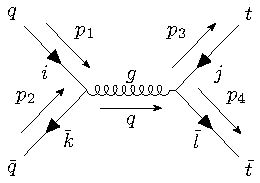
\includegraphics[width=0.75\textwidth]{figures/prob2QCDDiag.pdf}
	\end{subfigure}
	\begin{subfigure}[t]{0.45\textwidth}
		\centering
		\caption{QED $s$-channel diagram}
		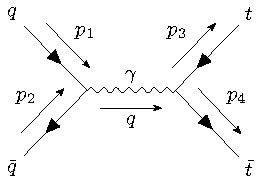
\includegraphics[width=0.75\textwidth]{figures/prob2QEDDiag.pdf}
	\end{subfigure}
	\caption{These are the $s$-channel diagrams for problem \ref{sec: 2}.}
	\label{fig: QCD feynman}
\end{figure}

\subsection{}
Coincidently, this is the same as slide 12 of the 11-02b lecture slides, since the initial state particles can have any of the three colors ($3^2 = 9$ color combinations), and the final state is the same way, but with color conserved:
\begin{align}
	\ev{\abs{C}^2} &= \frac{1}{9} \sum_{i,j,k,l=1}^3 \abs{C(ij \rightarrow kl)}^2,\\
	&= \frac{1}{9} \left[ 3\left(\frac{1}{3}\right)^2 +6\left(-\frac{1}{6}\right)^2 + 6\left(\frac{1}{2}\right)^2\right],\\
	&= \frac{2}{9}.
\end{align}

\subsection{}

\begin{align}
	E_{CM} &= 2m_t,\\
	E &= \frac{1}{2}E_{CM},\\
	&= m_t = 173\text{GeV}.
\end{align}

\subsection{}
\begin{align}
	\frac{\sigma(q\bar{q}\rightarrow t\bar{t})}{\sigma(e^+e^- \rightarrow t\bar{t})} &\approx \frac{\alpha_s^2 \ev{\abs{C}^2}}{\alpha_{EM}^2},\\
	&\approx 41.7.
\end{align}

% \nocite{*}
\printbib


\stopmcols


\end{document}

